\documentclass[12pt]{article}
\usepackage[english]{babel}
\usepackage{lingmacros}
\usepackage{tree-dvips}
\usepackage{amsmath, amsthm, amssymb}
\usepackage{graphicx}
\begin{document}


\title{Report: Seattle Car Accidents }
\author{Carlos Ríos} 
\date{\small{\today}}

\maketitle


\section*{}
\subsection*{Why? (Introduction)}
This work is aimed at society in general and the objective is to generate social awareness regarding traffic accidents, for that reason the language will be simple. Taking into account that traffic accidents represent the death of 1.3 million people around the world each year (World Health Organization), in this work it is intended to better understand this type of accidents, and evaluate which are the most relevant factors for their occurrence According to The World Health Organization, the victims (worldwide) correspond to passers-by in 50 \% of the cases, it is also explained that the majority of accidents in general occur due to human errors, however there are also environmental factors, such as automobile, or roads. Mainly we are going to use Machine Learning to create a model that classifies accidents according to their level of severity in order to predict the probability of an accident according to new features. \

\begin{figure}[htbp]
  \centering
    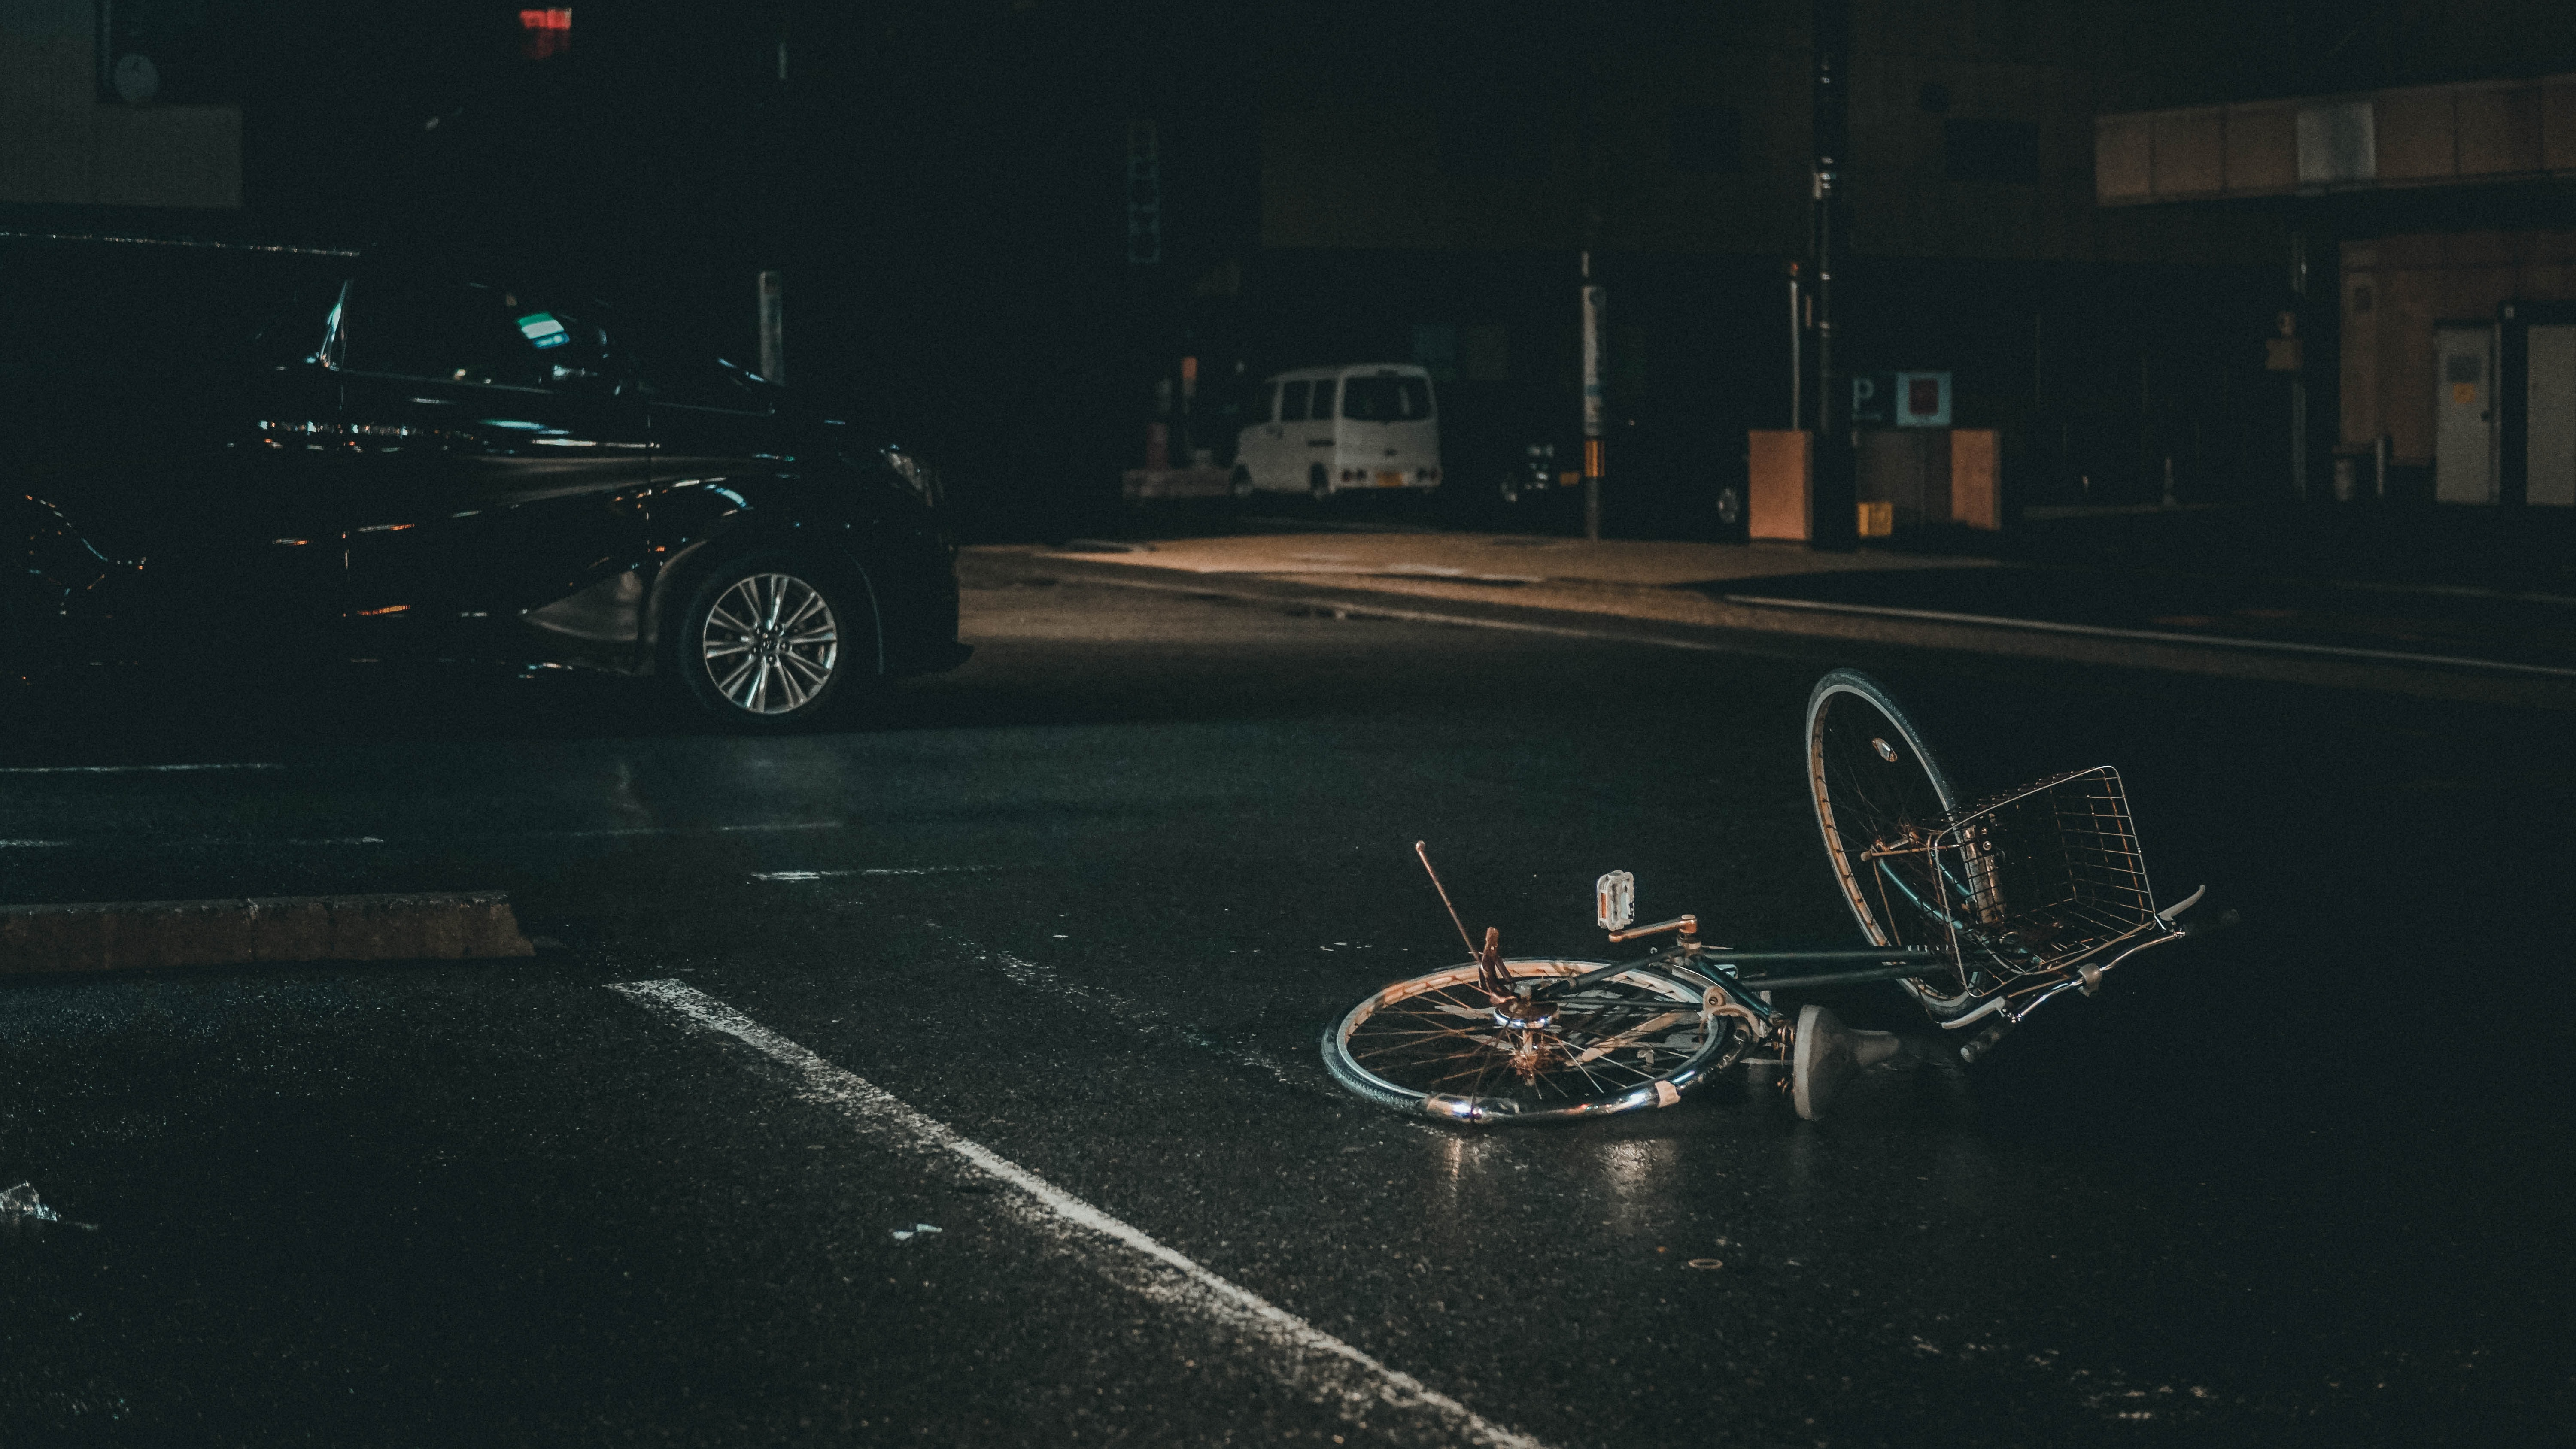
\includegraphics[width=1\textwidth]{../images/ian-valerio-9UxW_MqBGe4-unsplash.jpg}
  \caption{Photo by Ian Valerio on Unsplash.}
  \label{fig:intro}
\end{figure}




\subsection*{About data}
I will use the Collisions — All Years database provided by the Seattle SDOT Traffic Management Division. The data is made up of 194673 cases, and contains 38 features which I will separate into four groups:

a) There are some features that are not relevant for our purpose, for example those that correspond to identification codes (id), there are also repeated features or features with little information.

b) There are features that may not be relevant to apply machine learning techniques but that are relevant to better understand the problem, for example the location, coordinates and date.

c) On the other hand, there are those features that most likely have a strong influence on the severity of the accident. Even these have to be worked on because many contain a numerical code that does not refer to a numerical value but is an identification code for a certain type of accident. For this reason it is necessary to use a label encoder or a one hot encoder. Among them are: \\

\textbf{ADDRTYPE} It is the type of street it was on: Block, intersection or Alley. \\
\textbf{COLLISIONTYPE} This is the type of collision. \\
\textbf{PERSONCOUNT} It is the number of people involved in the collision. \\
\textbf{PEDCOUNT} It is the number of pedestrians involved. \\
\textbf{PEDCYLCOUNT} It is the number of cyclists involved in the collision. \\
\textbf{VEHCOUNT} It is the number of vehicles involved in the collision. \\
\textbf{JUNCTIONTYPE} Is the type of junction. \\
\textbf{UNDERINFL} If the person is under any alcoholic or narcotic influence. \\
\textbf{WEATHER} It's the weather. \\
\textbf{ROADCOND} It is the condition in which the road is contracted. \\
\textbf{LIGHTCOND} Describes the type of light that was present during the collision. \\
\textbf{SDOT COLCODE} It is an SDOT code that describes the collision. \\

\subsection*{Methodology and results}
I will explain the methodology and the results in a single subtitle as I will develop each part in sections.

  The first exploratory analyzes were, mainly, to count cases for each variable, it was found, for example, that in the majority of accidents two people are involved. I'll show the most interesting results I found, using histograms.


  The following analyzes were done: 1) Analyze the number of traffic accidents year by year. 2) Determine the days in which more accidents occur and in which fewer. 3) How accidents are distributed in the city. 4) What types of collisions occur the most? Which ones are the most injured? 5) Describe by means of a decision tree what factors are relevant for people to be injured in a traffic accident? \\

  1) The number of accidents were recorded year by year from 2004 to 2020. It can be seen that year by year there is a decrease in accidents, except for 2015, when there is a peak in property damage. On average, there are 3,590 injuries each year and 8,447 accidents involving property damage alone. In these mean values, the years 2004 and 2020 were omitted since there is no record of the complete years, Fig. \ref{fig:years}. \\

      

  \begin{figure}[htbp]
    \centering
      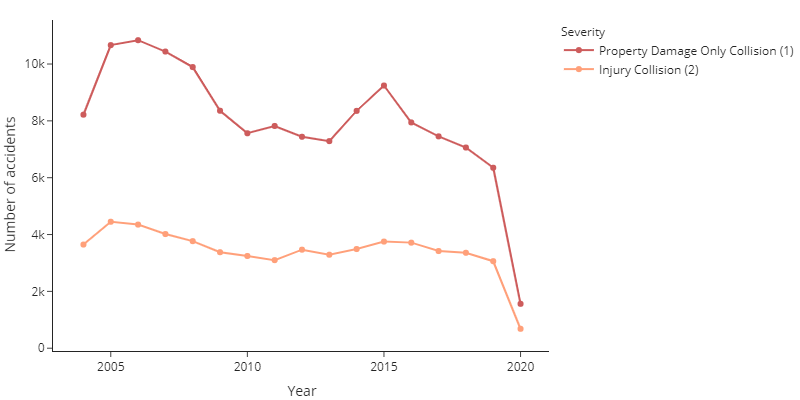
\includegraphics[width=1\textwidth]{../images/years.png}
    \caption{Car accidents year after year from 2004 to 2020.}
    \label{fig:years}
  \end{figure}


  2) The days with the most accidents were also counted. Without a doubt, the days in which accidents occur the most are on Fridays, as opposed to Sundays, when 20\% fewer accidents occurred, fig. \ref{fig:dayofweek}. \\
\begin{figure}[htbp]
    \centering
      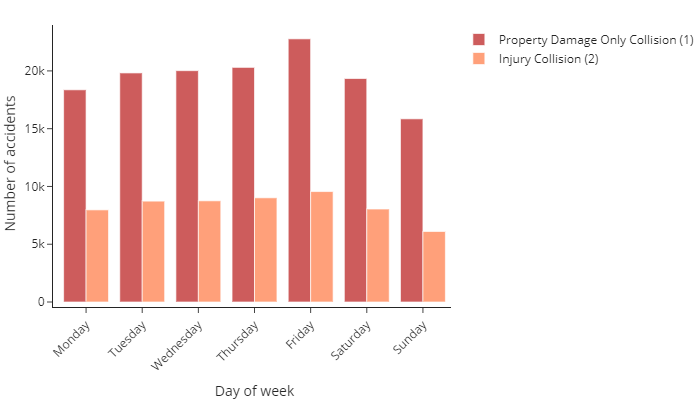
\includegraphics[width=1\textwidth]{../images/day_of_week.png}
    \caption{Histogram of car accidents by weekday.}
    \label{fig:dayofweek}
  \end{figure}
  
  3) The geospatial distribution gives us a better understanding of the accidents, fig. \ref{fig:map}. As you can see, this is a visualization of 7000 records obtained between 2004 and 2020 of accidents in Seattle (although there are more than 19000 records, the computation is quite heavy). The following graph shows how the accidents are distributed and from the shape of the streets I can infer that many more accidents occur in the urban center of the city than in the suburbs. \\

  \begin{figure}[htbp]
    \centering
      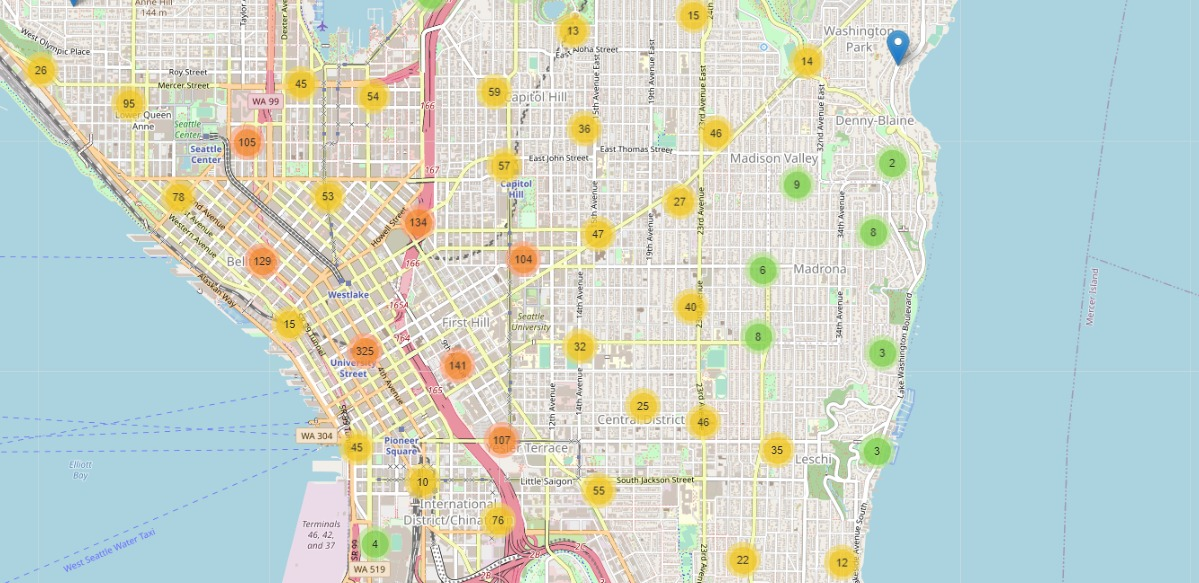
\includegraphics[width=1\textwidth]{../images/map_d.jpeg}
    \caption{Map of Seattle with car accidents. This map was generated with only 7000 data. }
    \label{fig:map}
  \end{figure}



  4) When counting the types of collisions we find that without a doubt most of the time that there is only material damage it is because the car was parked. However, injury accidents occur primarily because the collision was at an angle or because the car was rear-ended, fig. \ref{fig:collitiotype}. 

  I found the asymmetry between the number of crashes like turning right compared to turning left extremely curious. I was able to talk to a truck driver who traveled most of the highways in the US and he explained that it could be because when you turn right only one lane is involved, while when you turn left there are 3 lanes involved ( the opposite direction, the transversal and the opposite direction to the transversal) then for that reason many more accidents occur turning to the left than to the right. Although another possible explanation is the blind spots that cars have due to their very manufacture. \\


  \begin{figure}[htbp]
    \centering
      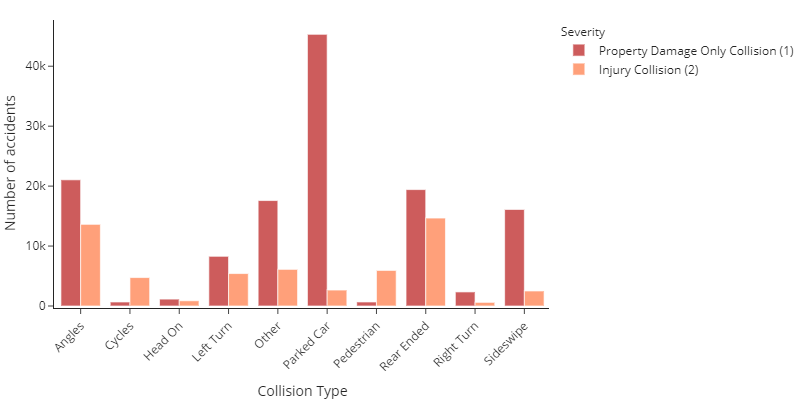
\includegraphics[width=1\textwidth]{../images/collition_type.png}
    \caption{Number of accidents by type of collision}
    \label{fig:collitiotype}
  \end{figure}
  5) Before analyzing the tree, it should be said that the variables were very slightly correlated, that is, there was no clear relationship between which was the most decisive factor for a collision with injuries or only material damage. The tree has an accuracy of 0.64 which can certainly be improved, fig. \ref{fig:tree}.

  What this tree wants to tell us is that if there are no cyclists or pedestrians, it is most likely that it is only material damage. While depending on the time of collision, the lights or the type of junction, there are more chances of accidents with injuries. On the right side, it tells us that if the number of people is greater than 6.5 and the number of vehicles involved is greater than 2.5, there is a high probability that they will be injured in the crash.\\

  \begin{figure}[htbp]
    \centering
      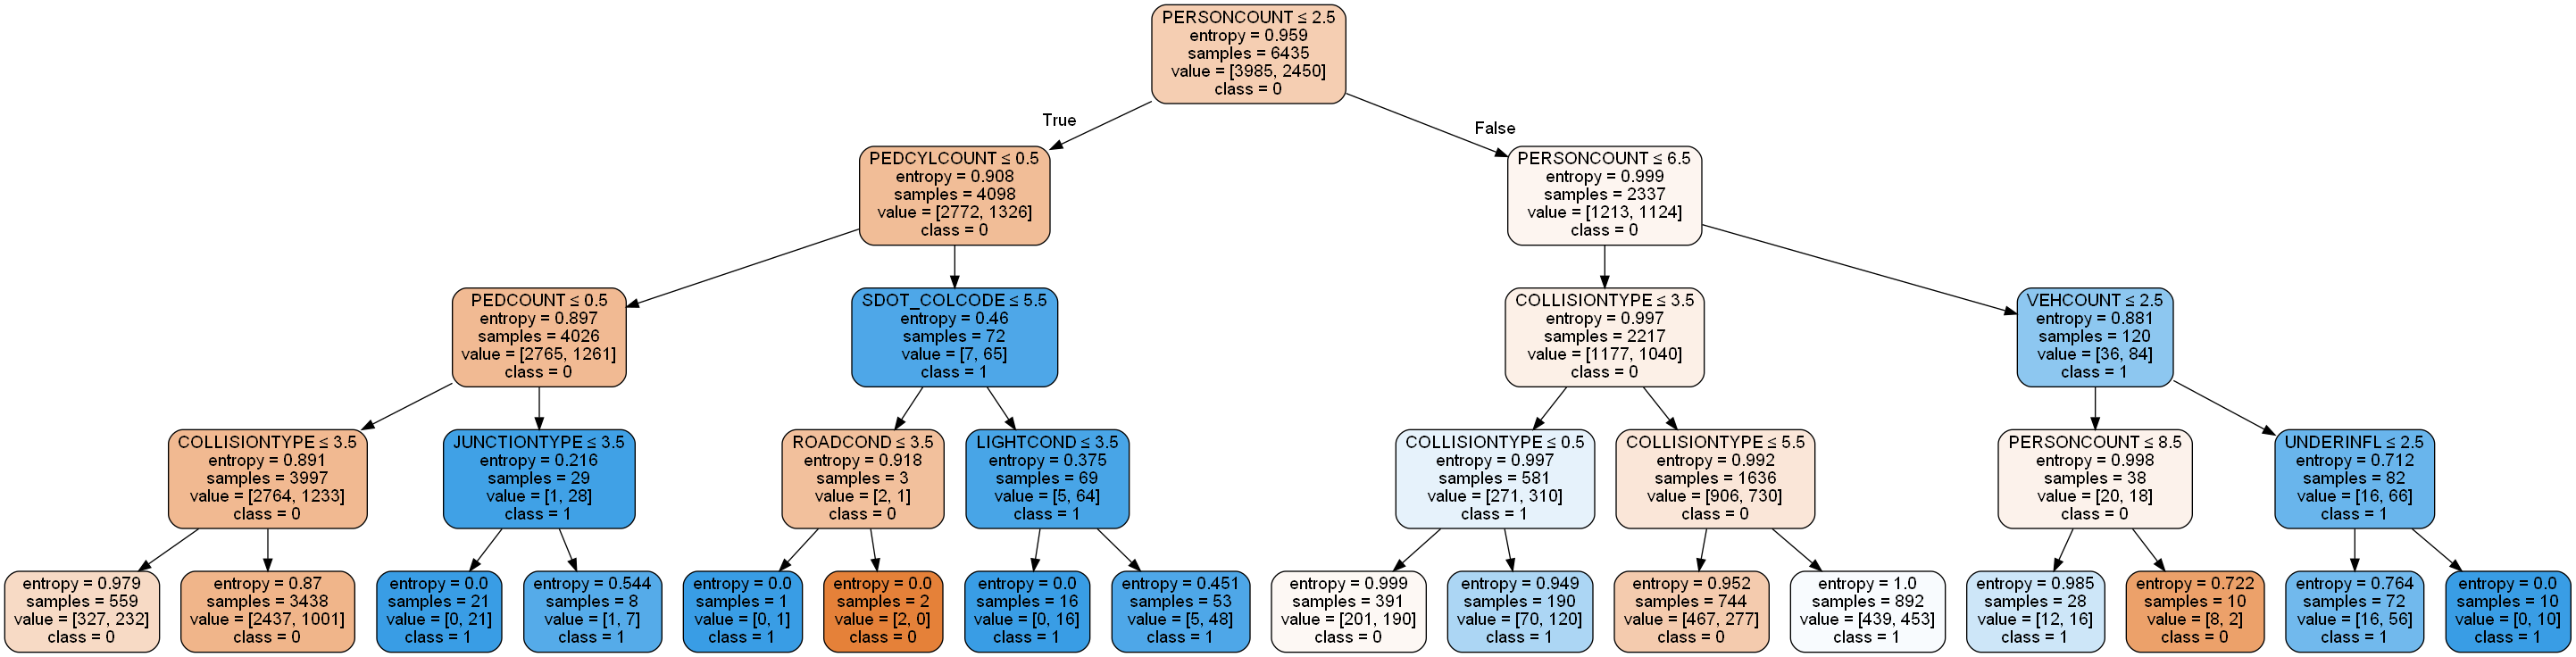
\includegraphics[width=1.5\textwidth, height=0.63\textwidth, angle=90]{../images/tree1.png}
    \caption{Decision tree using the most relevant parameters.}
    \label{fig:tree}
  \end{figure}

  \subsection*{Conclusions}

  Without a doubt, the tree could be improved with a better understanding of the features so we could have a more consistent label encoder.

   On the other hand, my suggestion is that you be more cautious on Fridays, do not leave your car parked anywhere, be more cautious when driving through the center and finally pay attention when you turn left!

  \subsection*{Acknowledgment}
  Victor Once - Comercial Driver. 
\end{document}